%
% Tesi D.S.I. - modello preso da
% Stanford University PhD thesis style -- modifications to the report style
%
%%%%%%%%%%%%%%%%%%%%%%%%%%%%%%%%%%%%%%%%%%%%%%%%%%%%%%%%%%%%%%%%%%%%%%%%%%%
%                                                                         %
%			TESI DOTTORATO                                                %
%			______________                                                %
%                                                                         %
%			AUTORE: Andrei Ciulpan                                        %
%                                                                         %
%			Ultima revisione: 14.05.2019                                  %
%                                                                         %
%%%%%%%%%%%%%%%%%%%%%%%%%%%%%%%%%%%%%%%%%%%%%%%%%%%%%%%%%%%%%%%%%%%%%%%%%%%
%
%
\documentclass[12pt]{report}
%    \renewcommand{\baselinestretch}{1.6}      % interline spacing
%
% \includeonly{}
%
%			PREAMBOLO
%
\usepackage[a4paper]{geometry}
\usepackage{amssymb,amsmath,amsthm}
\usepackage{graphicx}
\usepackage[hyphens,spaces,obeyspaces]{url}
\usepackage{hyperref}
\usepackage{epsfig}
\usepackage[italian]{babel}
\usepackage{tesi}
\usepackage{afterpage}
\usepackage{caption}
\usepackage{subcaption}

\addto{\captionsitalian}{%
	\renewcommand{\bibname}{Sitografia}
}

\newcommand\blankpage{%
	\null
	\thispagestyle{empty}%
	\addtocounter{page}{-1}%
	\newpage}

% per le accentate
\usepackage[utf8]{inputenc}
%
\newtheorem{myteor}{Teorema}[section]
%
\newenvironment{teor}{\begin{myteor}\sl}{\end{myteor}}
%
%
%			TITOLO
%
\begin{document}

\title{Sistema Accessi IoT}
\author{Andrei CIULPAN}
\dept{Corso di Laurea in Informatica} 
\anno{2018/2019}
\matricola{872394}
\relatore{Dott. Andrea TRENTINI}
\correlatore{Marco LANZA}
\afterpage{\blankpage}
% 
%			DEDICA
%
\beforepreface

{\hfill \footnotesize {\sl Ringrazio i miei genitori e la nonna per il sostegno e per la pazienza che hanno avuto.}}
\vskip 0.8cm
{\hfill \footnotesize {\sl Ringrazio i miei amici e compagni di università per aver reso l'esperienza più bella e soprattutto più facile.}}
\vskip 0.8cm
{\hfill \footnotesize {\sl Ringrazio i miei tutor e colleghi per avermi dato la possibilità di crescere e concludere la mia esperienza universitaria.}}
\vskip 0.8cm
{\hfill \footnotesize {\sl Un ringraziamento speciale a Elena per essere riuscita a farmi sorridere e a tirarmi su il morale in ogni giorno con la sua presenza nella mia vita.  Un altro ringraziamento a lei per la revisione della tesi.}}
       

\afterpreface


%			CAPITOLO 1: Intro
\chapter{Introduzione}\label{cap:introduzione}
%

Il controllo accessi è un sistema di protezione che permette l'accesso solo a determinate persone per via di qualche procedura di autenticazione: nel mondo fisico si può parlare di una semplice serratura (storicamente il sistema piu' utilizzato in assoluto) che può essere aperta solo dalle persone in possesso della chiave, mentre nel mondo dell'informatica si può notare l'enorme utilizzo delle procedure di autenticazione (login) che aiutano il sistema, tramite l'inserimento di un nome utente e password, a determinare automaticamente se una persona è autorizzata ad accedere alle risorse del sistema stesso.

Il controllo accessi\cite{controllo_accessi} è un tema molto sviluppato nel campo della sicurezza sia fisica che informatica: è stato segnalato che nel 2017, per il secondo anno consecutivo, il mercato del controllo accessi ha avuto la crescita piu' rapida nell'industria della sicurezza fisica\cite{crescita_controllo_accessi}. E' anche un sistema onnipresente, utilizzato in ospedali, fabbriche, supermercati, aziende, sistemi di trasporto pubblico (e.g l'ATM di Milano), case e tanti altri campi.  

La tesi si propone di trattare un sistema ibrido in cui il mondo fisico e il mondo informatico lavorano insieme: attraverso sensori ed attuatori è possibile avere la comunicazione tra i due mondi. 
Si tratta di un sistema IoT (Internet of Things), ovvero un sistema in cui la connessione Internet viene estesa anche al mondo degli oggetti fisici (smart objects\cite{smart_objects}) di uso comune. Gli oggetti si rendono riconoscibili e acquisiscono intelligenza grazie al fatto di possedere una o piu' delle seguenti funzionalità: identificazione, localizzazione, diagnosi di stato, interazione con l'ambiente circostante, elaborazione dati e ovviamente connessione.
Gli oggetti intelligenti di un sistema IoT sono normalmente dotati di un processore embedded, sensori e attuatori e sono in grado di agire sui dati raccolti dall'ambiente e, ancora piu' importante, mandare questi dati in rete dove possono poi essere analizzati\cite{IoT}. Un semplice esempio di un sistema IoT si può trovare in Figura \ref{fig:iot_diagram}.

Le seguente sezione di questo capitolo introdurrà il progetto stesso (denominato SimSim) che poi verrà dettagliato nei prossimi capitoli.

\begin{figure}
	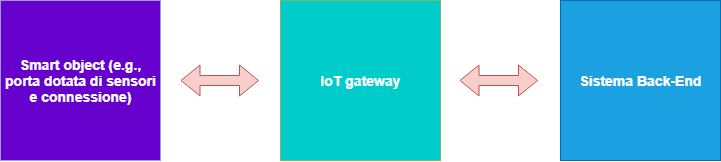
\includegraphics[width=\linewidth]{./img/iot_diagram.png}
	\caption{Esempio di sistema IoT}
	\label{fig:iot_diagram}
\end{figure}


%
\section{Requisiti del progetto}
%

L'attività principale del tirocinio è la realizzazione di un sistema di controllo accessi, da applicare presso varchi. Vengono elencati i requisiti del sistema:

\begin{enumerate}
	\item Deve essere in grado di funzionare con diverse modalità di riconoscimento:
	\begin{enumerate}
		\item Tessera RFID
		\item Tastierino numerico (password)
		\item Telecomando 
	\end{enumerate}
	\item Deve dare la possibilità di visualizzare su un display LCD ciò che sta succedendo (accesso consentito/negato ecc...). Inoltre deve essere implementata una funzione che permetta di visualizzare i codici delle tessere RFID sul display LCD (operazione protetta da una password).
	\item A seguito di ogni accesso avvenuto con successo deve aprire una porta (usando un servomotore) e salvare il log in un database remoto (in LAN) tramite WiFi.
	\item Deve avere un database per:
	\begin{enumerate}
		\item Tessere RFID
		\item Log degli accessi
		\item Soci
	\end{enumerate}
	\item Deve avere un'interfaccia grafica (in questo caso sito web) tramite la quale l'utente amministratore possa gestire il database con le seguenti funzioni: \begin{enumerate}
		\item Aggiungere/modificare/cancellare soci 
		\item Aggiungere/modificare/cancellare tessere 
		\item Visualizzare log
	\end{enumerate}
\end{enumerate}

I dispositivi scelti per soddisfare i requisiti sono stati un Arduino UNO (per la parte hardware) e un Raspberry Pi 3B+ su cui hostare il server. 
Nella figura \ref{fig:simsim} si può vedere una foto con il prototipo finito.
Nelle figure \ref{fig:usecase} e \ref{fig:flowchart} si possono trovare rispettivamente un diagramma dei casi d'uso e un diagramma di flusso del sistema.

\begin{figure}
	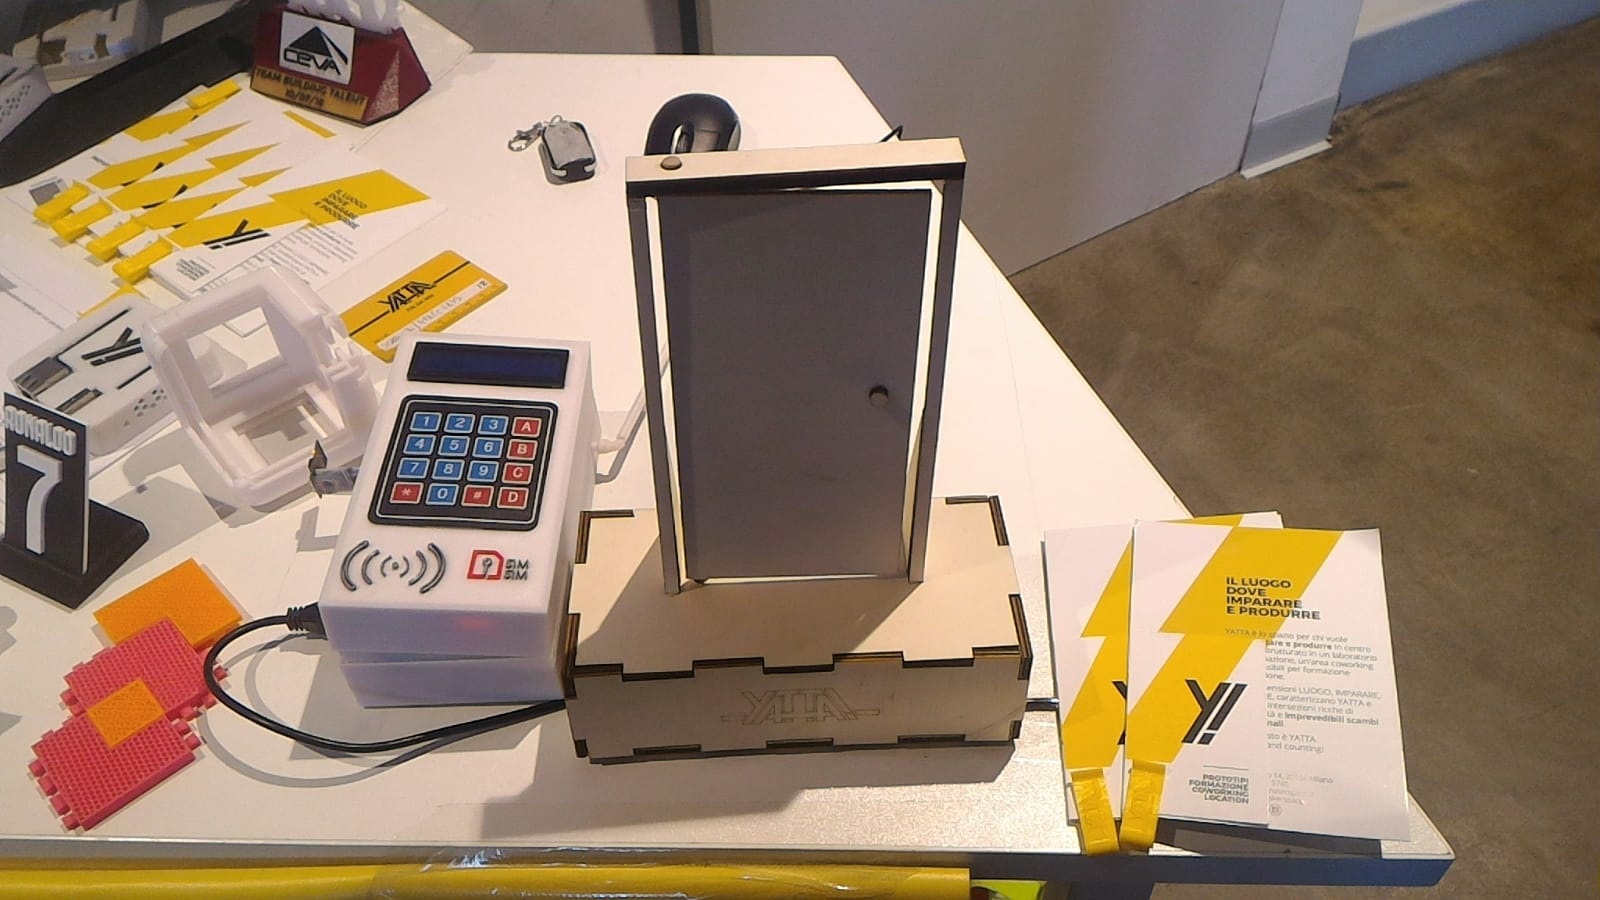
\includegraphics[width=1\linewidth]{./img/simsim.jpeg}
	\caption{SimSim}
	\label{fig:simsim}
\end{figure}

\begin{figure}
	\center{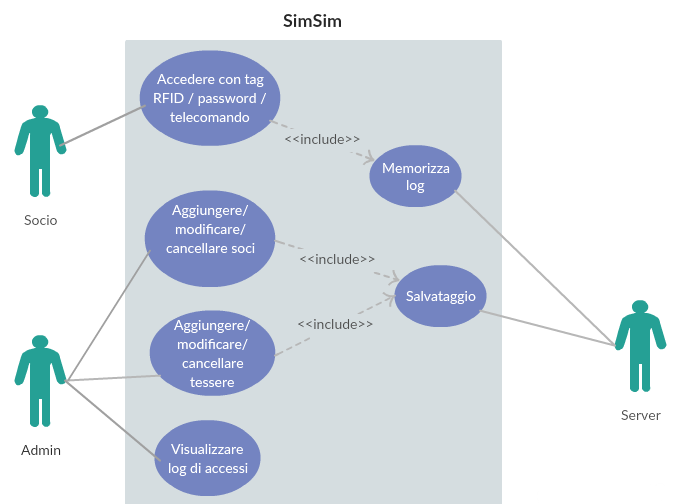
\includegraphics[width=0.6\linewidth]{./img/usecase.png}}
	\caption{Casi d'uso del sistema}
	\label{fig:usecase}
\end{figure}

\begin{figure}
	\center{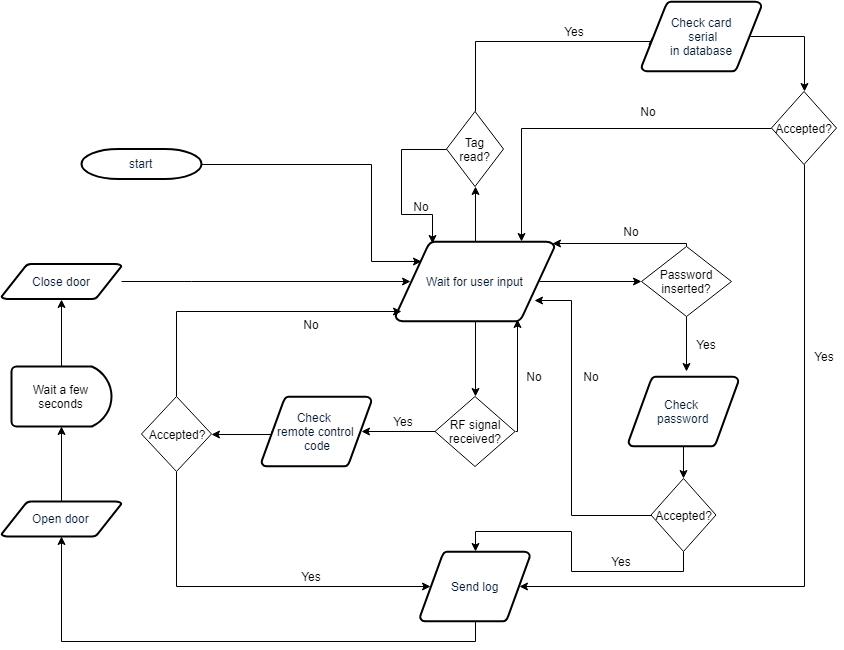
\includegraphics[width=0.9\linewidth]{./img/flowchart.png}}
	\caption{Diagramma di flusso del sistema}
	\label{fig:flowchart}
\end{figure}


%			CAPITOLO 2: Hardware
\chapter{Hardware}
\label{cap2}
%

In questo capitolo vengono dettagliati i dispositivi hardware utilizzati nel progetto. Uno schema completo del circuito elettrico si trova in Figura \ref{fig:schematics}.

\begin{figure}
	\center{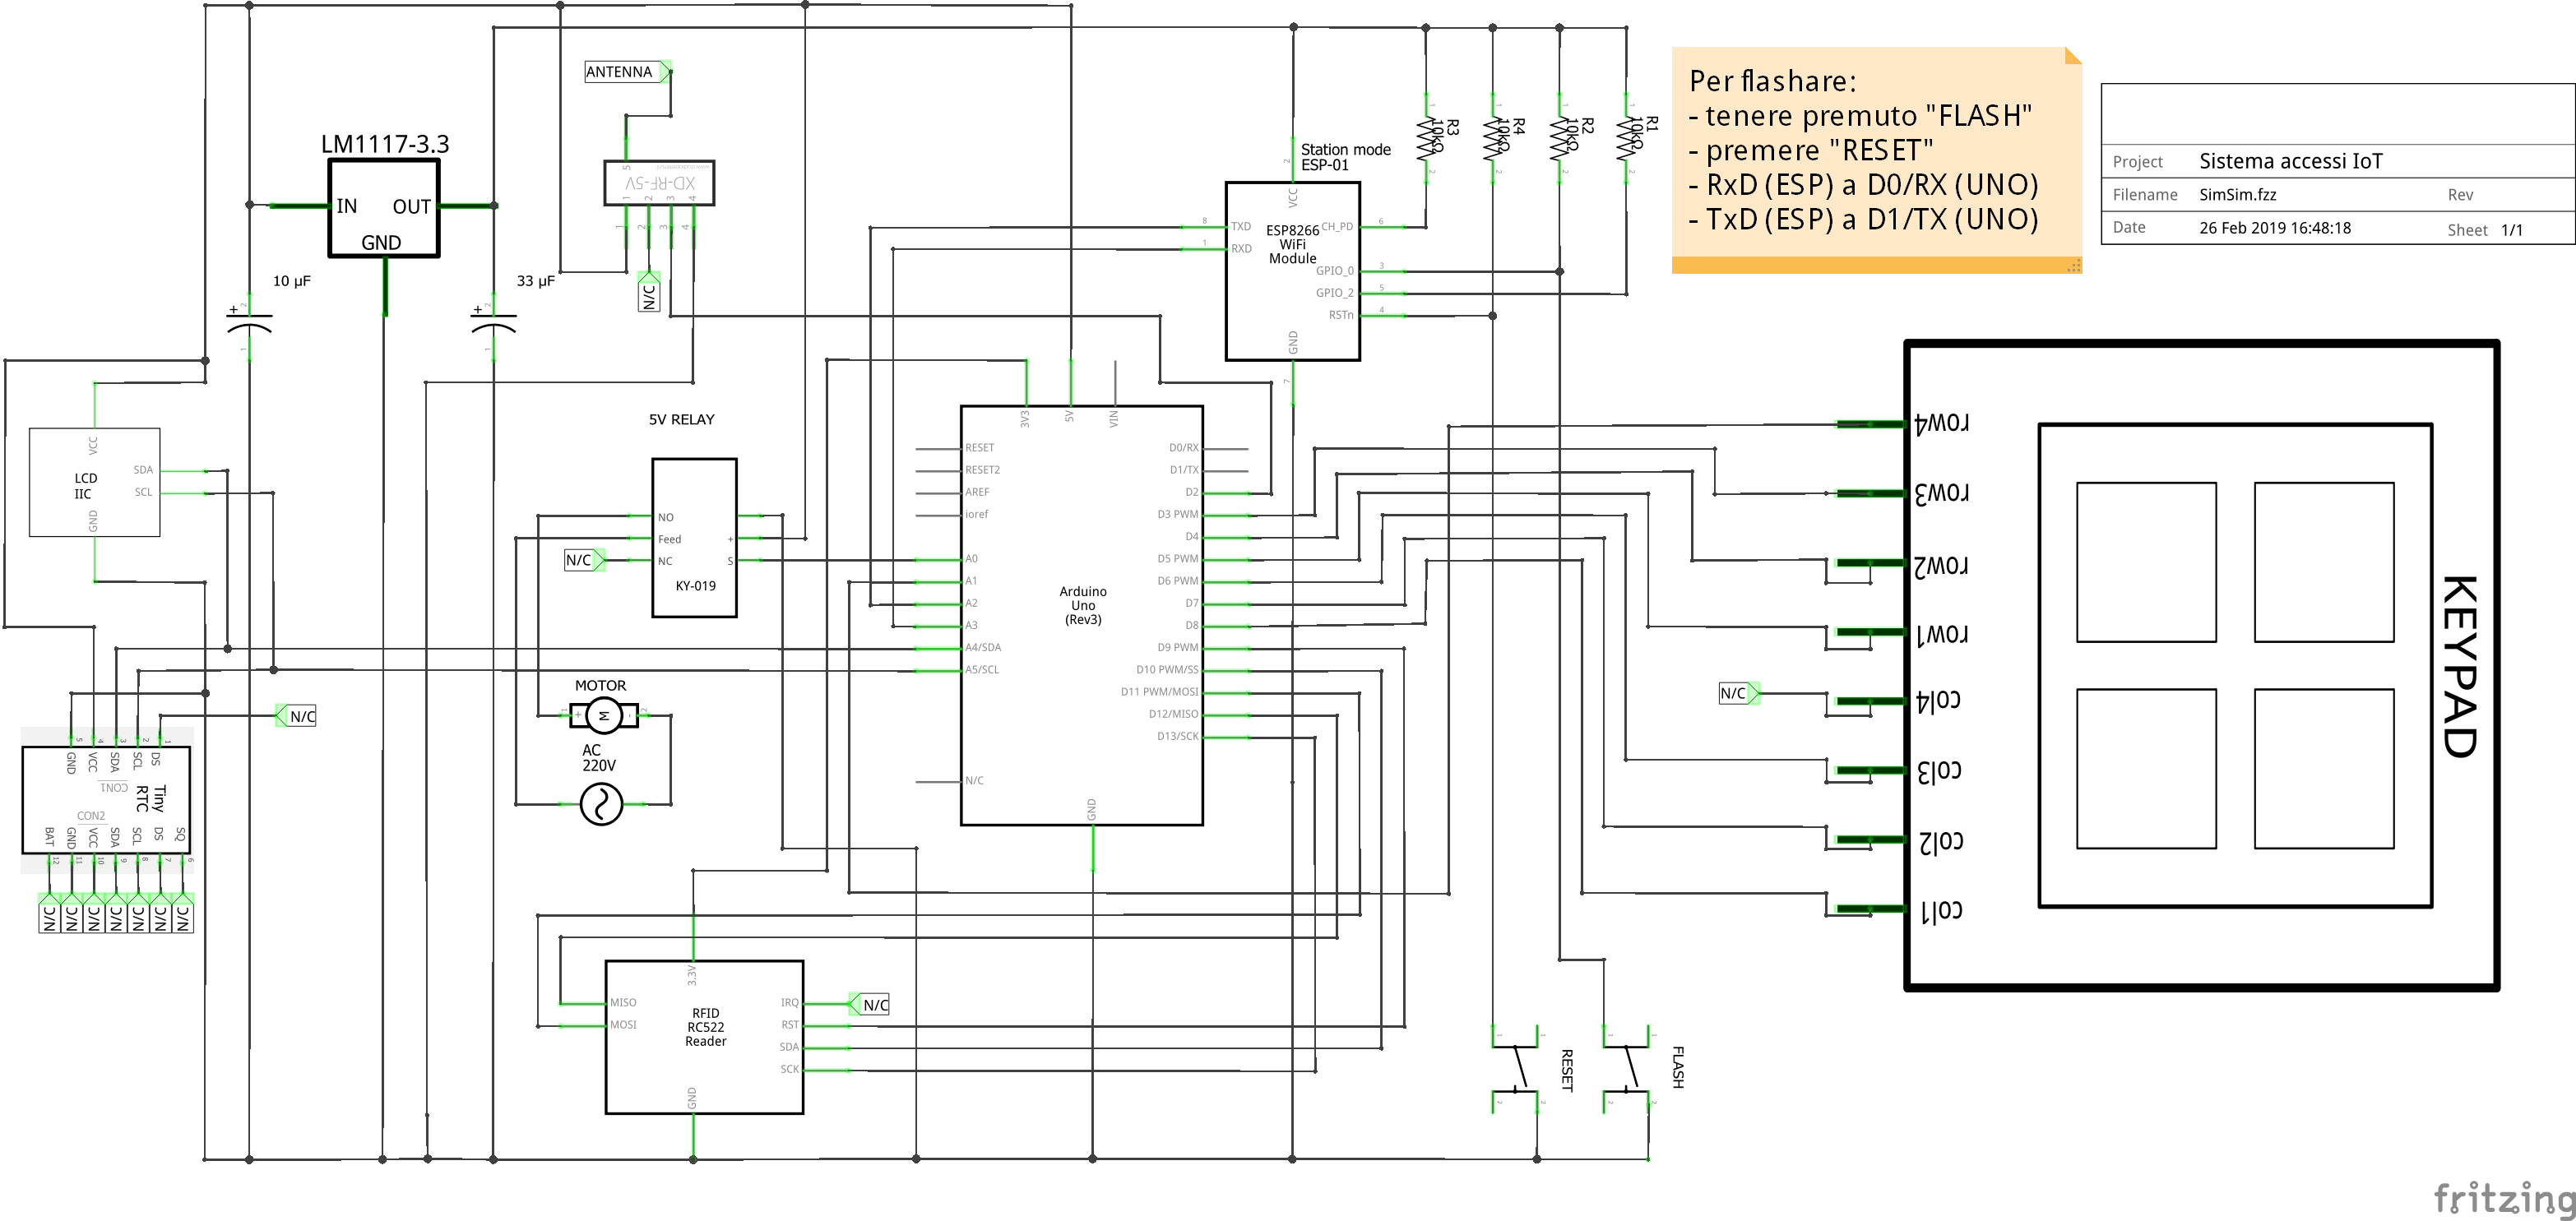
\includegraphics[width=\textwidth,height=1.1\textheight,keepaspectratio]{./img/schematics.png}}
	\caption{Schema del circuito}
	\label{fig:schematics}
\end{figure}


%
\section{Raspberry Pi}
%

Raspberry Pi (Figura \ref{fig:raspi}) è una serie di piccoli computer (system-on-chip) dalle dimensioni simili a quelle di una carta di credito. La scheda è stata sviluppata nel Regno Unito (Fondazione Raspberry Pi). Le prime versioni avevano poca potenza computazionale e sono state progettate con l'intenzione di offrire a insegnanti e studenti uno strumento semplice e poco costoso con cui poter insegnare e imparare a programmare. La scheda ha avuto un enorme successo anche in altri campi (e.g. robotica) e con ogni nuova versione è stata migliorata. Le ultime versioni sono assai potenti e possono essere utilizzate per tante altre cose. Le schede sono basate su sistemi operativi di tipo GNU/Linux, in particolare Raspbian che può essere scaricato dal sito della fondazione (\url{https://www.raspberrypi.org/downloads/}). 

La scheda utilizzata nel progetto (Raspberry Pi 3B+, \url{https://www.raspberrypi.org/products/raspberry-pi-3-model-b-plus/}) possiede un'architettura su 64 bit, essenziale per poter utilizzare in maniera efficiente MongoDB (che è limitato a una memoria di 2GB su un sistema a 32bit). Durante lo sviluppo del progetto ho scoperto che Raspbian in realtà non è stato ancora aggiornato per essere un sistema operativo a 64 bit, perciò non poteva sfruttare al meglio la scheda. Come soluzione a questo problema, è stato installato un sistema operativo chiamato openSUSE Tumbleweed (\url{https://software.opensuse.org/distributions/tumbleweed}) che funziona su architetture a 64 bit. 
La Raspberry Pi 3B+ possiede inoltre una scheda WiFi, il che la rende un buon candidato per lo scopo principale del progetto, ovvero quello di hostare il server.

\begin{figure}
	\center{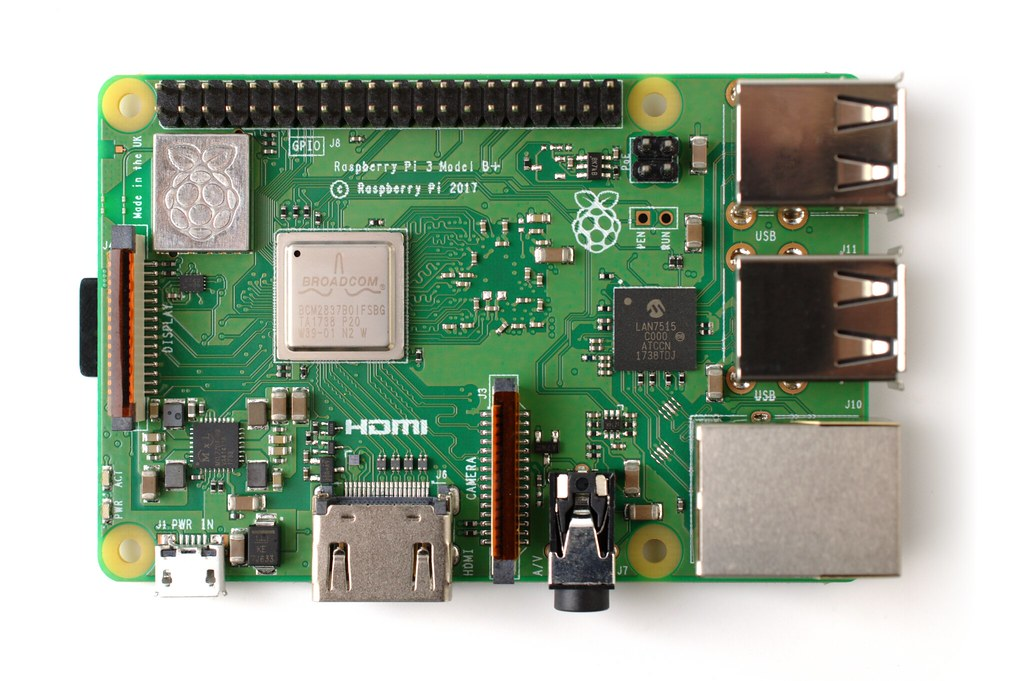
\includegraphics[width=0.4\linewidth]{./img/raspi.jpg}}
	\caption{Scheda Raspberry Pi}
	\label{fig:raspi}
\end{figure}

%
\section{Arduino UNO}
%

Arduino\cite{arduino_storia} è nata ad Ivrea nel 2005 come piattaforma di prototipazione elettronica di basso costo e open-source (dettaglio molto importante che ha portato al successo che ha avuto) che si basa su hardware e software flessibili e facili da usare. Il nome della scheda deriva di quello del bar di Ivrea frequentato dai fondatori del progetto ed la scheda è stata creata per artisti, designer e hobbisti. Essendo open-source, ha avuto un grande successo nel mondo degli hobbisti, anche a livello mondiale (tale da diventare una delle invenzioni piu' considerevoli nella storia dell'elettronica), grazie alla facilità di programmazione, basso costo e soprattutto disponibilità in rete delle informazioni necessarie per poter permettere a persone con grandi idee e poche capacità informatiche ed elettroniche di realizzare i propri progetti. 

Al giorno d'oggi Arduino potrebbe anche non essere la scelta immediata, anzi, ormai ci sono schede piu' potenti, piu' veloci e con migliori rapporti prestazioni/prezzo, ma non scordiamoci che è tutto grazie agli sviluppatori della scheda. Perchè scegliere, quindi, un Arduino? Essendo la scheda che ha fatto partire tutto, è anche la scheda piu' studiata e ciò significa che gira intorno a piu' informazioni, piu' librerie già pronte, piu' dispositivi compatibili e ha anche un sito di appassionati che si aiutano a vicenda dove si possono trovare tutorial, libri e tant'altro.

La scheda utilizzata nel progetto, Arduino UNO (Figura \ref{fig:uno}), è assolutamente la scheda piu' conosciuta al mondo e si può ormai trovare a dei prezzi molto bassi (ci sono tanti clone diversi in rete grazie al fatto di essere OpenHardware). Tra le varie caratteristiche vengono elencate le piu' interessanti:

\begin{itemize}
	\item Microcontrollore: ATmega328 (\url{https://www.sparkfun.com/datasheets/Components/SMD/ATMega328.pdf})
	\item Digital I/O Pins: 14 tra cui 6 offrono la funzione PWM (si veda la sezione \ref{sec:servomotore} "Servomotore") e 4 implementano il protocollo SPI (si veda la sezione \ref{sec:spi} "SPI")
	\item Analog I/O Pins: 6 tra cui 2 implementano il protocollo I$^2$C (si veda la sezione \ref{sec:i2c} "I$^2$C")
	\item Flash Memory: 32 KB
	\item EEPROM: 1 KB
	\item Clock Speed: 16 MHz
	\item DC Current per i pin I/O: max 40 mA
	\item DC Current per il pin 3V3: max 50 mA
	\item Operating Voltage: 5V
	\item Input Voltage (recommended): 7-12V
\end{itemize}

Tutto questo rende l'Arduino UNO un dispositivo ideale per il progetto. L'unica cosa che manca è la possibilità di accedere alla connessione WiFi, indispensabile per l'IoT, ma questo problema è stato risolto grazie ad un chip WiFi chiamato ESP8266 (si veda la sezione \ref{sec:esp8266} "ESP8266").

\begin{figure}
	\center{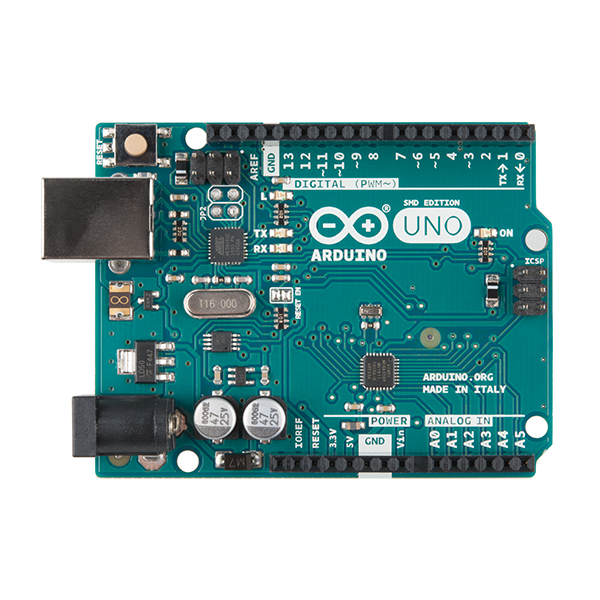
\includegraphics[width=0.4\linewidth]{./img/uno.jpg}}
	\caption{Scheda Arduino UNO}
	\label{fig:uno}
\end{figure}

%
\subsection{Arduino Programming Language}
%

La scheda Arduino UNO (e qualsiasi altra board compatibile con Arduino) può essere facilmente programmata utilizzando, ma non solo, l'Arduino IDE (Arduino Integrated Development Software), un software sviluppato da Arduino.cc e funzionante sulle 3 piattaforme dominanti (Windows, Linux e MacOS). Il linguaggio di programmazione si chiama "Arduino Programming Language"\cite{sistemi_embedded_atrent} ed è un derivato di Wiring (una piattaforma di sviluppo open-source composta da un linguaggio di programmazione, un IDE ed un circuito stampato basato su un microcontrollore). La sintassi è molto simile a quella del linguaggio C/C++; infatti il linguaggio Arduino è un insieme di funzioni e librerie C/C++ che possono essere chiamate dal codice. Forse la cosa diversa e che si nota di piu' rispetto ad altri linguaggi di programmazione è la diversa strutturazione dello sketch (sinonimo di programma): per poter funzionare vengono sempre definite due funzioni iniziali, setup() e loop(); la prima viene eseguita soltanto una volta all'avvio del programma e serve per dichiarare variabili, modalità dei pin (e.g input o output) ecc., mentre nella seconda viene messo il programma vero e proprio che viene eseguito ripetutamente... all'infinito.


%
\section{Real-time Clock}
%

I requisiti del progetto dicono che bisogna salvare un log dopo ogni accesso avvenuto con successo, e per fare ciò è necessario essere in grado di tenere traccia del tempo. La Raspberry Pi, diversamente dai PC a cui siamo abituati, può tenere traccia del tempo solo se ha accesso alla connessione Internet per accedere ad un server NTP (Network Time Protocol); nel progetto in questione, la Raspberry Pi, nonostante sia connessa alla rete LAN, è stata privata della connessione Internet per questioni di sicurezza (nessun utente esterno alla rete può accedere al server hostato in locale perciò elimina gran parte degli attacchi possibili). Ciò significa che per poter avere il cosidetto timestamp nei log bisogna trovare un modo di tenere traccia della data e dell'ora. Fortunatamente esistono dei piccoli chip chiamati RTC che fanno questo lavoro. 

In Figura \ref{fig:tinyRTC} si può vedere il dispositivo utilizzato nel progetto, chiamato TinyRTC; è un modulo basato sul clock chip DS1307 (\url{https://datasheets.maximintegrated.com/en/ds/DS1307.pdf}) e supporta il protocollo I$^2$C (si veda la sezione \ref{sec:i2c} "I$^2$C") per cui è facilmente utilizzabile dall'Arduino UNO.
L'orologio può essere programmato con data e ora corrente direttamente dal programma dell'Arduino e, grazie alla batteria al litio (CR1225), continua a tenere traccia del tempo anche senza alimentazione esterna. Il dispositivo è in grado di fornire con abbastanza precisione data e ora in termini di secondi, minuti, ora, giorno, mese e anno. Grazie alla popolarità di Arduino ci sono tante librerie per che permettono il facile utilizzo del dispositivo; io ho usato una libreria chiamata RTClib che si può trovare nel seguente repository: \url{https://github.com/adafruit/RTClib}. In Figura \ref{fig:tinyRTC_uno} si può vedere il collegamento con l'UNO.

\begin{figure}
	\centering
	\begin{minipage}{0.5\textwidth}
		\centering
		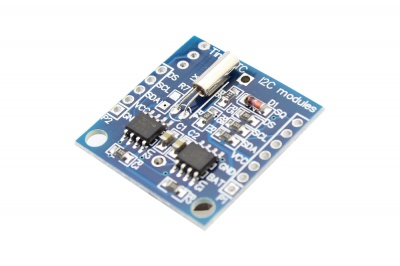
\includegraphics[width=0.5\linewidth]{./img/tinyRTC.jpg}
		\captionof{figure}{Tiny RTC}
		\label{fig:tinyRTC}
	\end{minipage}%
	\begin{minipage}{0.5\textwidth}
		\centering
		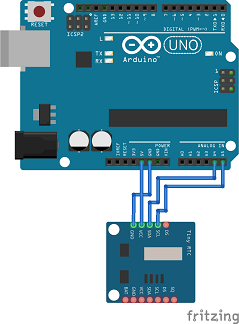
\includegraphics[width=0.5\linewidth]{./img/tinyRTC_uno.png}
		\captionof{figure}{Tiny RTC e Arduino UNO}
		\label{fig:tinyRTC_uno}
	\end{minipage}
\end{figure}

%
\section{Trasmettitore-ricevitore RF}
%

Ci sono due principali tipi di tecnologie per i telecomandi: a raggi infrarossi o a radio-frequenza (RF).
La tecnologia a raggi infrarossi è quella piu' utilizzata ed è usata da tanti dispositivi elettronici (un esempio molto comune è il telecomando della TV). In questo caso trasmettitore e ricevitore devono essere messi "faccia-a-faccia" e non troppo distanti tra di loro, perciò non è il caso di usare questa tecnologia nel progetto (non si potrebbe, ad esempio, aprire la porta stando dietro ad un muro).

La tecnologia scelta è quindi quella a radio-frequenza, in cui trasmettitore e ricevitore possono comunicare anche se sono messi in camere diverse. Il dispositivo scelto (MX-05V/XD-RF-5V, Figura \ref{fig:rx_tx_module}) è un modulo composto da trasmettitore e ricevitore in radio-frequenza a 433 MHz (\url{https://sites.google.com/site/summerfuelrobots/arduino-sensor-tutorials/rf-wireless-transmitter-receiver-module-433mhz-for-arduino}). Il trasmettitore è stato utilizzato soltanto per programmare i telecomandi dell'azienda con i codici voluti grazie alla loro funzione di clonazione (codice in Figura \ref{fig:clone_code}). Il ricevitore, invece, è sempre collegato all'Arduino (Figura \ref{fig:rf_uno}) e riesce a ricevere i segnali mandati dai telecomandi anche da qualche decine di metri di distanza. Se il codice che viene mandato dal telecomando è corretto allora l'Arduino lo risconosce e apre la porta, altrimenti fa finta di niente. 


Il ricevitore, per aumentare il range, è stato accoppiato con un'antenna lunga 17,3 cm. Il motivo di questa scelta è che la lunghezza dell'antenna deve essere 1/4 di quella della lunghezza d'onda. Bisogna quindi calcolare la lunghezza d'onda $\lambda$:
%
\[\lambda(m) = \frac{v(m/s)}{f(Hz)} = \frac{299,792,458}{433,000,000} = 0,692 m\] 
%
dove \textit{v} è la velocità della luce e \textit{f} è la frequenza (433 MHz). Ora si può trovare la lunghezza dell'antenna: 
%
\[\frac{\lambda}{4} = \frac{0,692}{4} = 0,173m = 17,3 cm \]
%

\begin{figure}
	\center{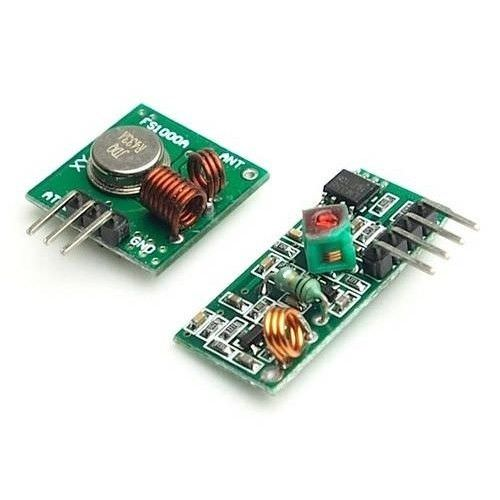
\includegraphics[width=0.3\linewidth]{./img/receiver_transmitter_module.jpg}}
	\caption{Modulo transceiver MX-05V/XD-RF-5V}
	\label{fig:rx_tx_module}
\end{figure}

\begin{figure}
	\center{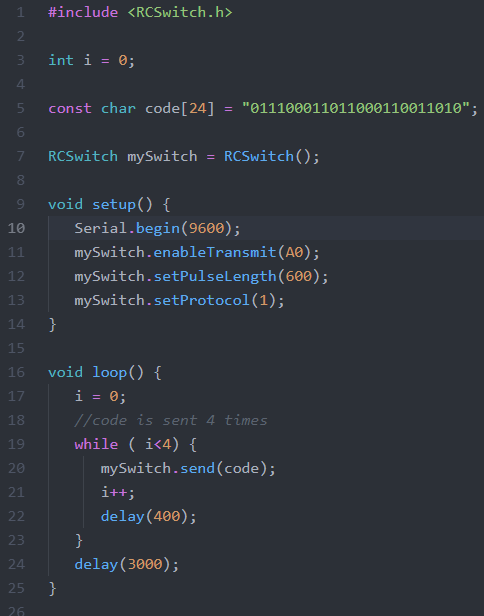
\includegraphics[width=0.45\linewidth]{./img/clonare_telecomando.png}}
	\caption{Programma di Arduino per mandare i codici che poi vengono clonati dai telecomandi}
	\label{fig:clone_code}
\end{figure}

\begin{figure}
	\center{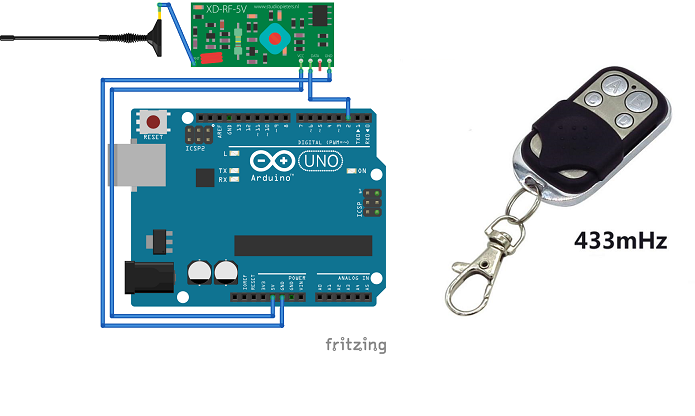
\includegraphics[width=0.5\linewidth]{./img/rf_uno.png}}
	\caption{RF Receiver + Telecomando e Arduino UNO}
	\label{fig:rf_uno}
\end{figure}

\pagebreak

%
\section{Servomotore}\label{sec:servomotore}
%

Esistono tanti tipi diversi di motori Arduino-compatibili, ognuno con i propri punti forti e deboli, perciò bisogna valutare bene quale scegliere in base alle necessità del progetto. In questo caso il lavoro del motore è semplice: deve girare la serratura di una porta da una parte e dall'altra, quindi senza particolare precisione, velocità o potenza. Siccome non c'è nemmeno il bisogno di avere una rotazione completa (bastano 180$^{\circ}$), è immediato pensare al servomotore che è anche facilmente controllabile da un Arduino grazie ai suoi pin PWM e alla libreria Servo (\url{https://www.arduino.cc/en/reference/servo}).

Il servomotore (Figura \ref{fig:servo}) è un dispositivo elettromeccanico a basso consumo energetico ed è costituito da un motore DC, un gruppo di ingranaggi, un circuito di controllo (un ponte-H integrato) e un contenitore di plastica che lo racchiude.
La particolarità del servomotore è che può ruotare con una precisione di alcuni gradi (normalmente da 0$^{\circ}$ a 180$^{\circ}$) in base alla larghezza dell'impulso che riceve. Questa tecnica si chiama Pulse Width Modulation (PWM) e consiste in una serie di impulsi di larghezza variabile che determinano la posizione del servo.

\begin{figure}
	\center{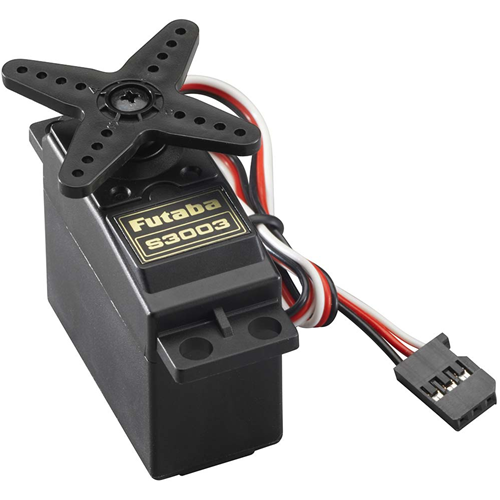
\includegraphics[width=0.15\linewidth]{./img/servo.png}}
	\caption{Servomotore}
	\label{fig:servo}
\end{figure}

%
\subsection{PWM}
%

\textbf{P}ulse \textbf{W}idth \textbf{M}odulation è una tecnica che consiste in una serie di impulsi di larghezza variabile che determinano la posizione del servo. E' quindi un modo di ricavare un risultato analogico a partire da un segnale digitale. Un segnale PWM ha una forma d'onda quadra, con periodo fisso, ma spesso non simmetrica: la durata della semi-onda alta può variare (si veda la Figura \ref{fig:pwm}). La durata \textit{T[ON]} del segnale alto viene misurata in percentuale e si chiama duty cycle: ad esempio un duty cycle del 25\% significa che \textit{T[ON]} dura per 1/4 della durata del periodo fisso \textit{T}. Questo tipo di segnale non è un vero e proprio segnale analogico, però può essere interpretato tale: quello che succede è che la tensione viene applicata e levata nel giro di frazioni di secondo perciò quello che si chiama "tensione efficace" è in realtà minore della tensione reale applicata. Per calcolare la tensione efficace \textit{Veff} basta sapere la tensione applicata \textit{Vcc} e il duty cycle \textit{DC} (che si trova facendo il rapporto tra \textit{T[ON]} e \textit{T}):

%
\[Veff = Vcc \cdot DC\]
%
Nel grafico della Figura \ref{fig:pwm} la \textit{Veff} è rappresentata dalla linea orizzontale che copre il segnale digitale.

\begin{figure}
	\center{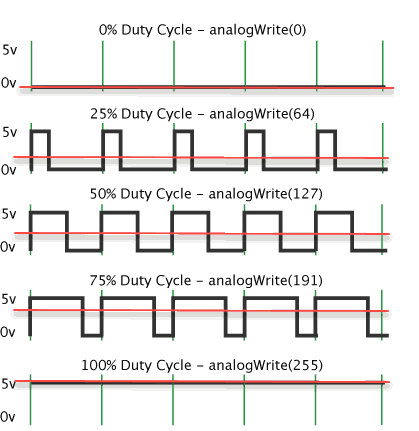
\includegraphics[width=0.4\linewidth]{./img/pwm.png}}
	\caption{Segnali PWM e comando analogWrite(int value) per generarli con l'Arduino}
	\label{fig:pwm}
\end{figure}

Generalmente, nel caso dei servomotori, si ha un periodo totale \textit{T} = 20 ms, perciò ogni 20 ms il servo riceve un nuovo impulso. La posizione del motore dipende quindi dalla durata del tempo \textit{T[ON]} che questo impulso rimane ad un livello logico HIGH. Nel grafico della Figura \ref{fig:servo_pwm} si nota che la durata dell'impulso alto è un valore compreso tra 1ms (Duty Cycle = 5\%) e 2ms (Duty Cycle = 10\%). Fissata la posizione centrale del servo a 90$^{\circ}$, allora abbiamo che: 


\begin{figure}
	\center{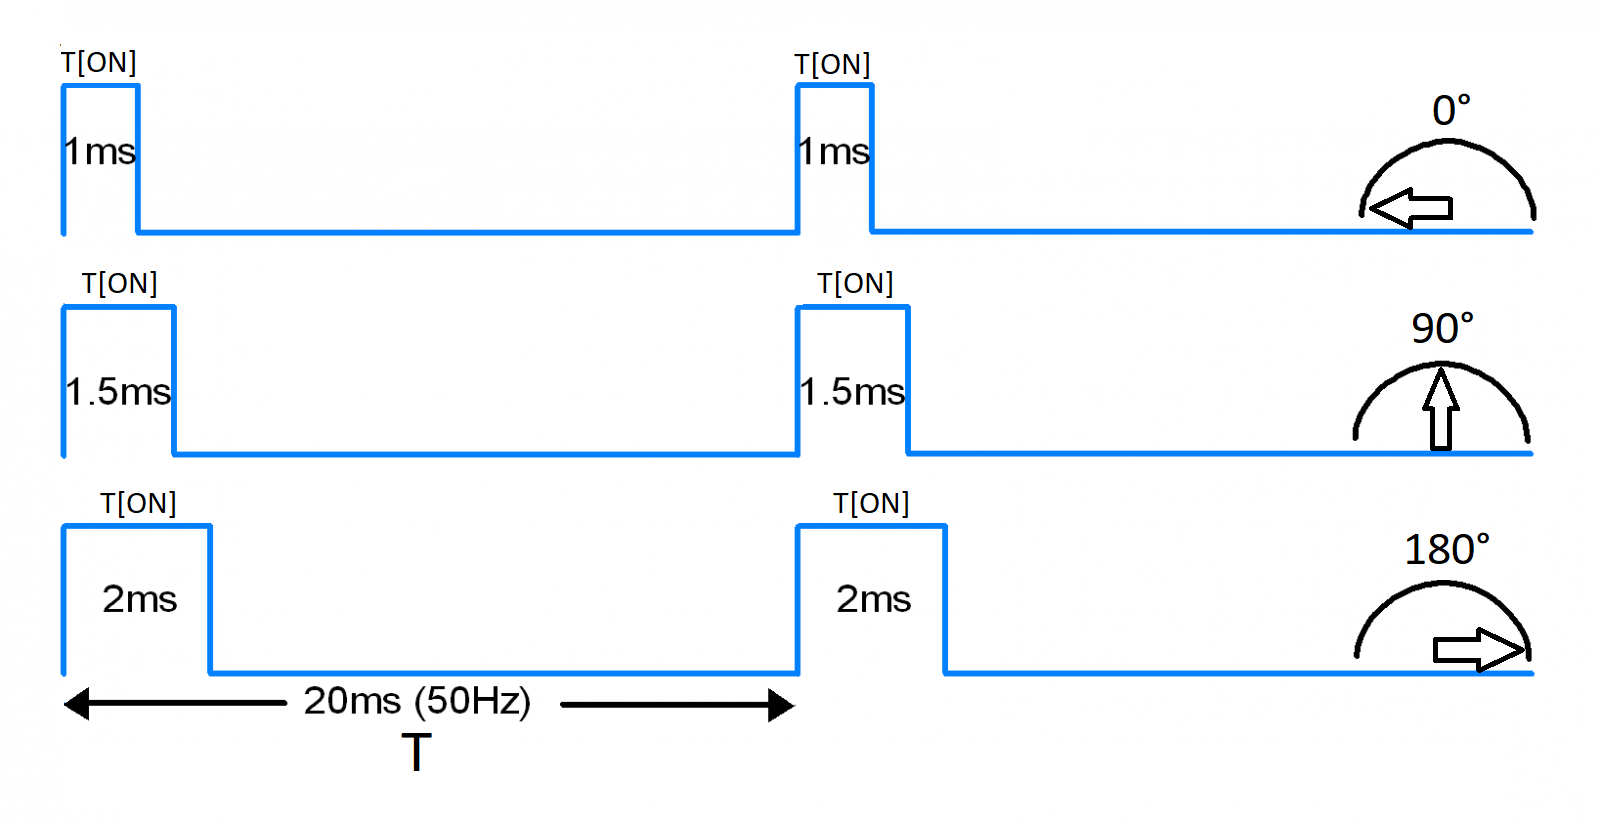
\includegraphics[width=0.9\linewidth]{./img/servo_pwm.png}}
	\caption{Segnali PWM nel servomotore}
	\label{fig:servo_pwm}
\end{figure}


\begin{itemize}
	\item se la durata del livello logico HIGH dell'impulso sta nell'intervallo [1ms, 1.5ms] allora il servo ruota verso sinistra a partire dalla posizione centrale (la sua posizione varia tra 0$^{\circ}$ e 90$^{\circ}$)
	\item se la durata del livello logico HIGH dell'impulso è uguale a 1.5ms allora il servo resta fermo a 90$^{\circ}$
	\item se la durata del livello logico HIGH dell'impulso sta nell'intervallo [1.5ms, 2ms] allora il servo ruota verso destra a partire dalla posizione centrale (la sua posizione varia tra 90$^{\circ}$ e 180$^{\circ}$)
\end{itemize}

Per controllare un servomotore con l'Arduino non dobbiamo pensare a tutte queste cose perchè esiste una libreria (\url{https://www.arduino.cc/en/reference/servo}) che ne facilita il lavoro: basta pensare in gradi (esempio di collegamento tra servo e Arduino in Figura \ref{fig:servo_uno} e di codice in Figura \ref{fig:servo_code}).

\begin{figure}
	\center{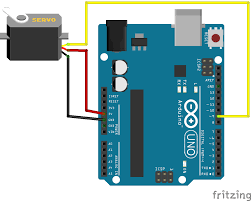
\includegraphics[width=0.3\linewidth]{./img/servo_uno.png}}
	\caption{Servomotore e Arduino UNO}
	\label{fig:servo_uno}
\end{figure}

\begin{figure}
	\center{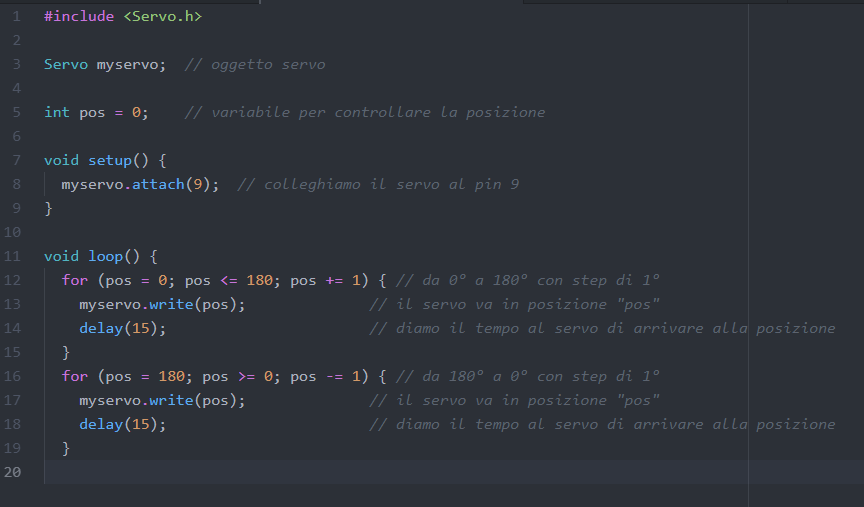
\includegraphics[width=0.9\linewidth]{./img/servo_code.png}}
	\caption{Codice per controllare un servomotore tramite la libreria "servo.h"}
	\label{fig:servo_code}
\end{figure}

%
\section{RFID Reader}
%

\textbf{R}adio \textbf{F}requency \textbf{ID}entification (RFID) è un termine utilizzato per descrivere tecnologie contactless che fanno uso delle onde radio per identificare oggetti, persone e animali sia da vicino (tag passivi) che da lontano (tag attivi). L'identificazione è resa possibile grazie ad un lettore RFID in grado di interrogare i cosidetti tag, ovvero dei dispositivi elettronici di varie forme e dimensioni che possiedono i dati necessari per l'identificazione e che principalmente si dividono in due categorie: 

\begin{itemize}
	\item I tag passivi sono poco costosi e contengono un'antenna e un piccolo chip con identificativo univoco e privo di alimentazione. Questi tag vengono utilizzati per l'identificazione a breve distanza (qualche centimetro) e vengono "attivati" dalle onde radio del lettore.
	\item I tag attivi sono piu' costosi e permettono, grazie all'alimentazione interna (emettono loro stessi i segnali radio), l'identificazione a lunga distanza (fino a 200 metri).
\end{itemize}

La tecnologia RFID si diversifica anche nella frequenza utilizzata e trova utilizzo in tanti campi diversi quali gestione accessi, tracciabilità degli animali, gestione dei biglietti elettronici, ecc$.$ (per le basse e medie frequenze), ma anche in Telepass, identificazione di auto in movimento, tracciabilità degli oggetti in movimento ecc. (per le frequenze alte e altissime).

\begin{figure}
	\center{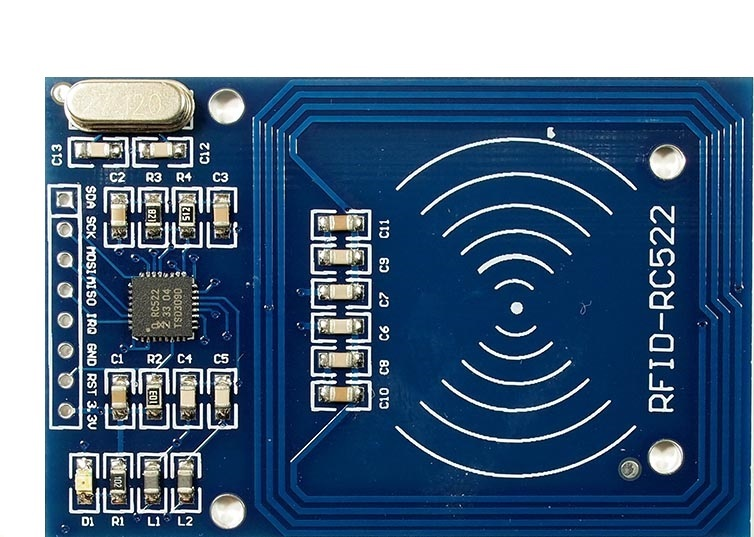
\includegraphics[width=0.35\linewidth]{./img/mfrc522.jpg}}
	\caption{Lettore RFID MFRC522}
	\label{fig:mfrc522}
\end{figure}

Il lettore RFID utilizzato nel progetto è il MFRC522 (\url{https://www.nxp.com/docs/en/data-sheet/MFRC522.pdf}; Figura \ref{fig:mfrc522}). Esso opera su una frequenza di 13.56 MHz ed è in grado di comunicare con tag che si conformano allo standard ISO/IEC 14443 A/MIFARE. Implementa vari protocolli di comunicazione (SPI, Serial UART, I$^2$C) ma è stata sviluppata solo una libreria di Arduino (\url{https://github.com/miguelbalboa/rfid}) basata sul protocollo SPI (si veda la sezione \ref{sec:spi} "SPI").

Nelle Figure \ref{fig:rfid_uno} e \ref{fig:rfid_code} si trovano rispettivamente il circuito per collegare il lettore RFID con l'UNO e un esempio di codice per la lettura dei tag.

\begin{figure}
	\center{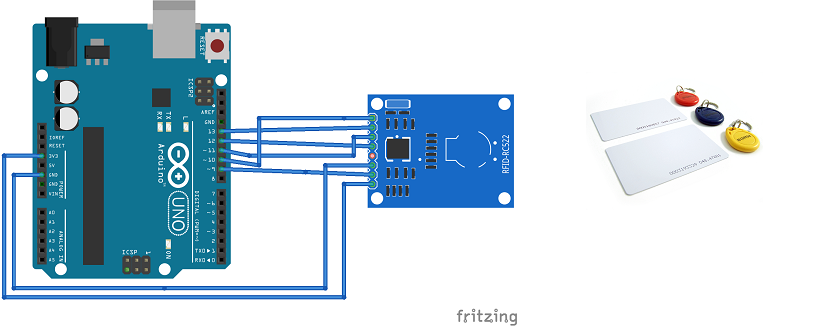
\includegraphics[width=0.65\linewidth]{./img/rfid_uno.png}}
	\caption{RFID + Tag e Arduino UNO}
	\label{fig:rfid_uno}
\end{figure}

\begin{figure}
	\center{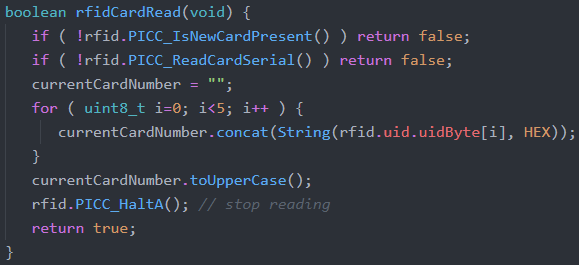
\includegraphics[width=0.75\linewidth]{./img/rfid_code.png}}
	\caption{Esempio di codice in Arduino per la lettura dei tag}
	\label{fig:rfid_code}
\end{figure}

%
\section{Display LCD 16x2}
%

I moduli LCD trovano ampio utilizzo nei sistemi embedded grazie al basso costo, disponibilità e utilità. Il display utilizzato si chiama "16x2 LCD" (Figura \ref{fig:16x2}) proprio perchè possiede uno schermo su cui si possono scrivere 2 linee di 16 caratteri ciascuna. Questi dispositivi sono abbastanza complessi (ci sono 1280 pixel da indirizzare) e per poterli utilizzare in maniera semplice ed efficiente è necessario avere un'interfaccia. Infatti i display LCD spesso vengono accoppiati con un controller che rende la vita facile al programmatore. Il controller piu' utilizzato (infatti è considerato uno standard \textit{de facto}) si chiama HD44780 (\url{https://www.sparkfun.com/datasheets/LCD/HD44780.pdf}), costruito dalla Hitachi, ed è in grado di controllare display LCD capaci di visualizzare solo caratteri. L'HD44780 supporta il trasferimento parallelo a 8 bit (possiede 8 bit di dati) e il suo compito principale è di ricevere i comandi e i dati in arrivo dall'MCU per poi processarli
e mandarli all'LCD.

\begin{figure}
	\center{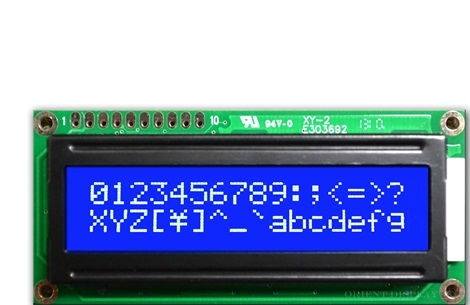
\includegraphics[width=0.6\linewidth]{./img/16x2.jpg}}
	\caption{Display LCD 16x2}
	\label{fig:16x2}
\end{figure}

\begin{figure}
	\center{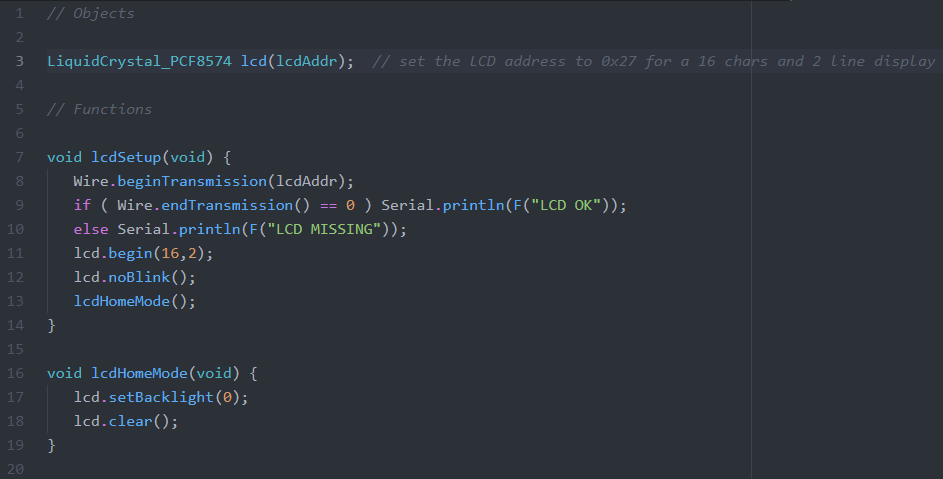
\includegraphics[width=0.9\linewidth]{./img/lcd_code.png}}
	\caption{Esempio di codice per utilizzare il LCD 16x2 con la libreria LiquidCrystal\_PCF8574)}
	\label{fig:lcd_code}
\end{figure}

Il problema principale dell'LCD 16x2, come si può vedere nella Tabella \ref{tab:lcd_pinout}, è il numero di pin necessari da collegare (e la pazienza per farlo) all'Arduino per poter farlo funzionare correttamente. Questo significa che, siccome l'Arduino ha un numero limitato di pin (13 digitali e 6 analogici), essi potrebbero non bastare per un progetto di dimensioni piu' grandi. Fortunatamente c'è una soluzione: I$^2$C (si veda la sezione \ref{sec:i2c} "I$^2$C"). Esiste un chip che rende possibile la riduzione del numero di pin utilizzati a 2 (SDA e SCL) cambiando l'interfaccia parallela del controller in una seriale. Questo chip si chiama PCF8574 I/O Expander ed è definito come un backpack (è letteralmente uno "zaino" che si salda sopra l'LCD) e permette appunto all'LCD e all'Arduino di comunicare utilizzando il protocollo I$^2$C. Per utilizzarlo con Arduino esiste già una libreria che si chiama LiquidCrystal\_PCF8574 (\url{https://platformio.org/lib/show/1165/LiquidCrystal_PCF8574/installation}) che sfrutta la libreria Wire (\url{https://www.arduino.cc/en/Reference/Wire}) per implementare alcune funzioni utili al programmatore (esempio di codice in Figura \ref{fig:lcd_code}).


\begin{table}[h!]
	\begin{center}
		\begin{tabular}{l|l} 
			\textbf{Pin} & \textbf{Funzione del pin} \\
			\hline
			1 & Vss (GND) \\
			2 & Vcc (5V) \\ 
			3 & Vee (Contrasto) \\
			4 & RS (Register Select: 0 per selezionare l'invio di un comando, 1 per i dati) \\
			5 & R/W (Read/Write: 0 per la scrittura di dati/comandi, 1 per la lettura dati/stato) \\
			6 & E (Enable bit: inizia il ciclo di scrittura o lettura) \\
			7 & D0 (Data 0) \\
			8 & D1 (Data 1) \\
			9 & D2 (Data 2) \\
			10 & D3 (Data 3) \\
			11 & D4 (Data 4) \\
			12 & D5 (Data 5) \\
			13 & D6 (Data 6) \\
			14 & D7 (Data 7) \\
			15 & A (Anodo (+): retroilluminazione) \\
			16 & K (Catodo (-): retroilluminazione) \\
		\end{tabular}
	\caption{Pinout di un display LCD 16x2 con il controller HD44780}
	\label{tab:lcd_pinout}
	\end{center}
\end{table}

%
\section{Keypad}
%

\begin{figure}
	\centering
	\begin{subfigure}{.5\textwidth}
		\centering
		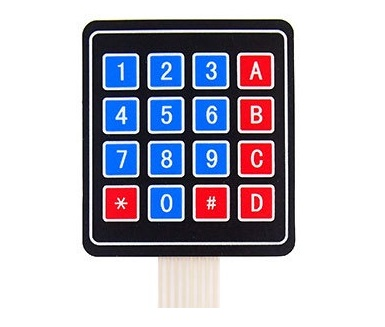
\includegraphics[width=0.8\linewidth]{./img/keypad.jpg}
		\caption{Tastierino 4x4}
		\label{fig:keypad}
	\end{subfigure}%
	\begin{subfigure}{.5\textwidth}
		\centering
		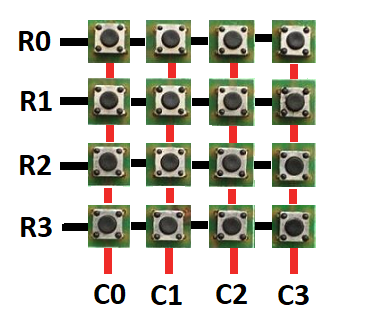
\includegraphics[width=0.78\linewidth]{./img/keypad_matrix.png}
		\caption{Rappresentazione a matrice dei pulsanti}
		\label{fig:keypad_matrix}
	\end{subfigure}
	\caption{Keypad}
	\label{fig:keypad_both}
\end{figure}

I tastierini sono dei dispositivi di input ampiamente utilizzati per dare la possibilità alle persone di interagire con un sistema (e.g. inserire una password, controllare un robot ecc.). Normalmente i tasti sono disposti in un formato a matrice (in questo caso 4x4, ovvero 16 pulsanti) e permettono ad un microcontrollore di capire facilmente quale tasto è stato premuto in base alle linee che si attivano: nella Figura \ref{fig:keypad_both} si può facilmente vedere che premendo il pulsante "2" vengono attivate le linee "R0" e "C1" e il microcontrollore, grazie a come è stato programmato (esempio di configurazione in Figura \ref{fig:keypad_config}), è in grado di dire che quel pulsante specifico è stato premuto. Le funzioni per utilizzare il tastierino sono implementate nella libreria Keypad di Arduino (\url{https://playground.arduino.cc/Code/Keypad/}). Nella Figura \ref{fig:keypad_uno} si può vedere un esempio di collegamento tra il tastierino e l'Arduino UNO.


\begin{figure}
	\center{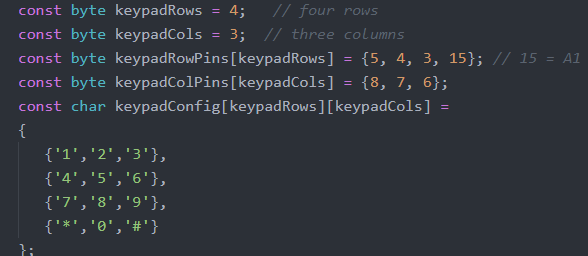
\includegraphics[width=0.9\linewidth]{./img/keypad_config.png}}
	\caption{Esempio di configurazione in Arduino della tastiera (in questo caso non viene utilizzata l'ultima colonna con le lettere)}
	\label{fig:keypad_config}
\end{figure}

\begin{figure}
	\center{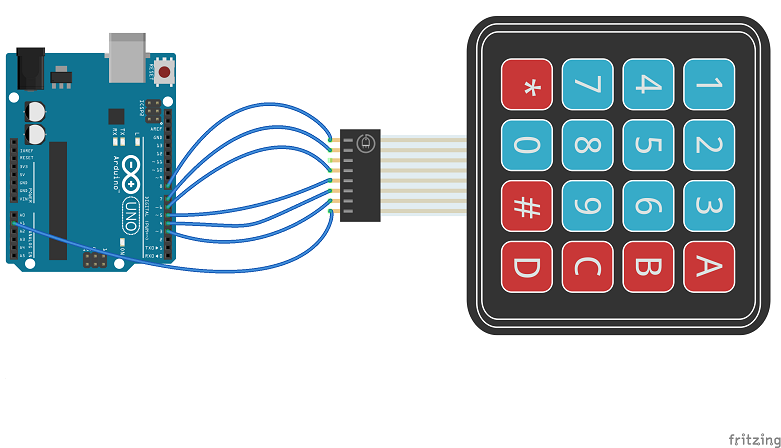
\includegraphics[width=0.5\linewidth]{./img/keypad_uno.png}}
	\caption{Keypad e Arduino UNO}
	\label{fig:keypad_uno}
\end{figure}


%
\section{ESP8266}\label{sec:esp8266}
%

L'Arduino UNO, a differenza di altre board piu' recenti, non ha il WiFi incorporato perciò bisogna accoppiarlo con uno shield che gli permette di avere quella funzionalità necessaria per un progetto IoT. Per questo progetto è stata scelta l'ESP8266, una famiglia di microchip WiFi a basso costo prodotta da Espressif Systems. Il dispositivo usato in realtà si chiama ESP-01 (Figura \ref{fig:esp01}), è basato sul modulo ESP8266 ed è prodotto da terze parti (Ai-Thinker). Questo piccolo modulo permette a microcontrollori di connettersi alla rete WiFi per fare semplici chiamate HTTP.
Tra le varie caratteristiche vengono elencate le piu' interessanti:

\begin{figure}
	\center{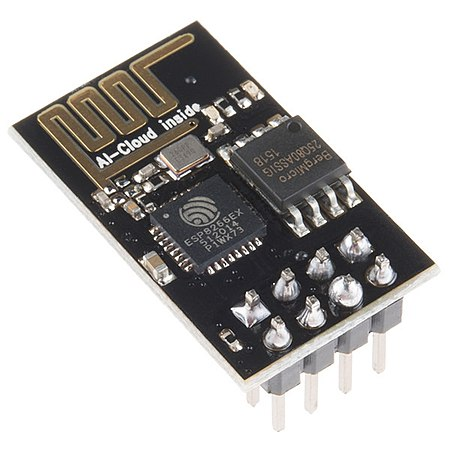
\includegraphics[width=0.2\linewidth]{./img/esp01.jpg}}
	\caption{L'ESP-01 di Ai-Thinker}
	\label{fig:esp01}
\end{figure}


\begin{itemize}
	\item basso costo e molto compatto
	\item antenna incorporata nel PCB
	\item 512 KB flash memory su cui caricare il programma
	\item 80 KB user data RAM
	\item può essere usato sia come Station che come Access Point (AP)
	\item implementa la funzione Deep Sleep per evitare il consumo eccessivo durante l'inattività
	\item può essere programmato attraverso l'IDE di Arduino
	\item implementa il protocollo IEEE 802.11 b/g/n
\end{itemize}
Il pinout e le funzioni dei pin si trovano rispettivamente in Figura \ref{fig:esp_pinout_img} e in Tabella \ref{tab:esp01_pinout}. 

L'ESP-01 va alimentato a una tensione di 3.3V ma secondo il datasheet (\url{http://www.microchip.ua/wireless/esp01.pdf}) potrebbe richiedere anche fino a 170mA di corrente perciò non si può alimentare direttamente dal piedino 3V3 dell'Arduino perchè non eroga abbastanza corrente (max 50 mA secondo \url{https://store.arduino.cc/arduino-uno-rev3}). Per questo motivo è stato usato il pin 5V dell'Arduino collegato ad un regolatore di tensione (LM1117, \url{http://www.ti.com/lit/ds/symlink/lm1117.pdf}). 
Il circuito si può trovare in Figura \ref{fig:esp_uno}.

\vspace{\baselineskip}
\begin{minipage}{\textwidth}
	\begin{minipage}[b]{0.35\textwidth}
		\centering{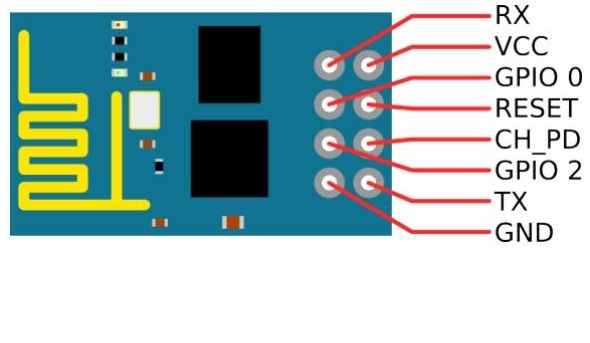
\includegraphics[width=1\linewidth]{./img/esp_pinout_img.jpg}}	
		\captionof{figure}{ESP-01 Pinout}
		\label{fig:esp_pinout_img}
	\end{minipage}
	\hfill
	\begin{minipage}[b]{0.65\textwidth}
		\centering
		\begin{tabular}{l|l}
			\textbf{Pin} & \textbf{Funzione del pin} \\
			\hline
			1 & RX (Receive data bit) \\
			2 & GPIO0 (General Purpose Input/Output Pin) \\
			3 & GPIO2 (General Purpose Input/Output Pin) \\
			4 & GND \\
			5 & VCC (+3.3V) \\
			6 & RST (Reset chip) \\
			7 & CH\_PD (Chip power-down) \\
			8 & TX (Transmit data bit) \\
		\end{tabular}
		\captionof{table}{Funzioni dei pin dell'ESP-01}
		\label{tab:esp01_pinout}
	\end{minipage}
\end{minipage}
\vspace{\baselineskip}

\begin{figure}
	\center{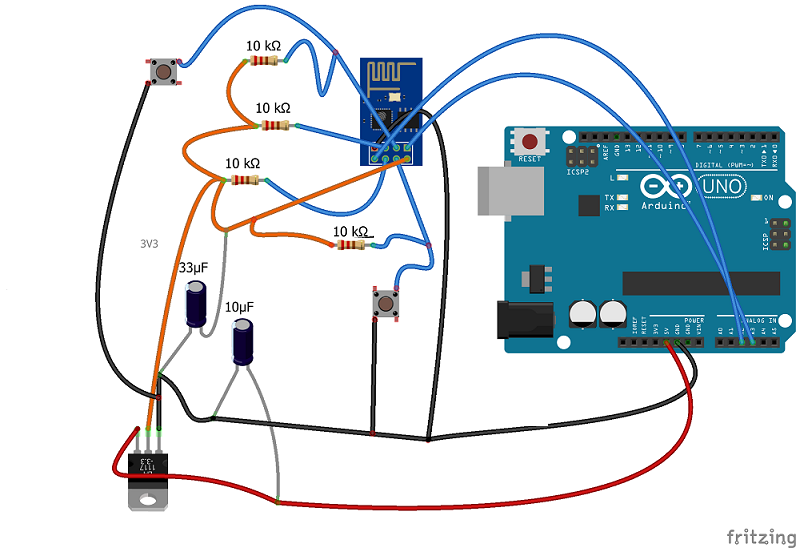
\includegraphics[width=0.7\linewidth]{./img/esp_uno.png}}
	\caption{ESP-01 e Arduino UNO}
	\label{fig:esp_uno}
\end{figure}


Il dispositivo viene pre-programmato con il firmware AT  (\url{https://www.electrodragon.com/w/ESP8266\_AT-Command\_firmware}) ma è possibile programmarlo anche con codice proprio (vedere Tabella \ref{tab:esp01_modes} per le modalità di funzionamento) utilizzando l'IDE di Arduino. Nella Figura \ref{fig:esp01_flashed_code} si può vedere una parte del codice caricato sull'ESP-01: all'accensione non fa altro che connettersi alla rete WiFi locale.

Dopo aver effettuato la connessione, l'ESP-01 si mette in ascolto sulla porta seriale per dati in arrivo dall'Arduino (Figura \ref{fig:esp01_listen}) per poi eseguire varie funzioni in base alla richiesta.


\begin{table}[h!]
	\begin{center}
		\begin{tabular}{l|l} 
			\textbf{GPIO-0} & \textbf{Modalità} \\
			\hline
			GND & Flash mode (modalità programmazione) \\
			VCC & Normal mode (il chip esegue il codice caricato) \\
		\end{tabular}
		\caption{Modalità di funzionamento dell'ESP-01}
		\label{tab:esp01_modes}
	\end{center}
\end{table}

\begin{figure}
	\center{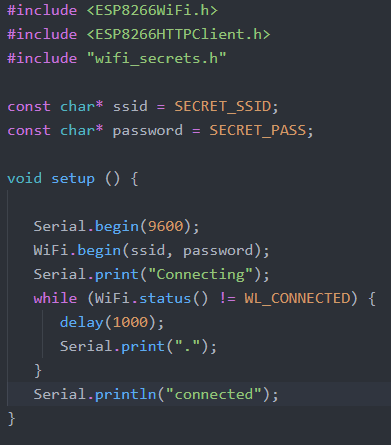
\includegraphics[width=0.5\linewidth]{./img/esp01_flashed_code.png}}
	\caption{Snippet del codice caricato sull'ESP-01. La libreria utilizzata è molto bene documentata e si trova a \url{https://arduino-esp8266.readthedocs.io/en/latest/esp8266wifi/readme.html})}
	\label{fig:esp01_flashed_code}
\end{figure}

\begin{figure}
	\center{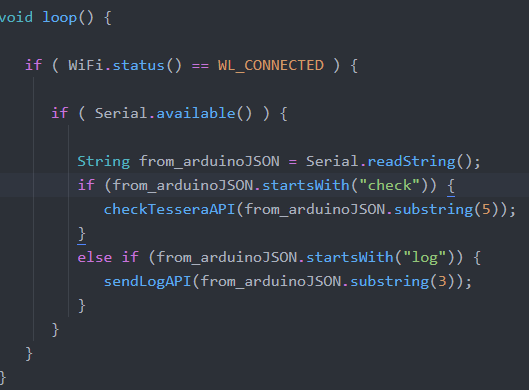
\includegraphics[width=0.5\linewidth]{./img/esp01_listen.png}}
	\caption{Snippet del codice caricato sull'ESP-01}
	\label{fig:esp01_listen}
\end{figure}

L'Arduino è programmato per mandare 2 tipi di richieste: 

\begin{itemize}
	\item "check" per quando deve inoltrare all'ESP-01 il codice del tag letto (Figura \ref{fig:uno_check})
	\item "log" per quando deve inoltrare all'ESP-01 un log (Figura \ref{fig:uno_log})
\end{itemize}

\begin{figure}
	\centering
	\begin{subfigure}{0.5\textwidth}
		\centering
		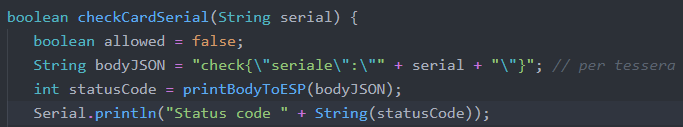
\includegraphics[width=0.99\linewidth]{./img/uno_check.png}
		\caption{Funzione per verificare un tag}
		\label{fig:uno_check}
	\end{subfigure}%
	\begin{subfigure}{0.5\textwidth}
		\centering
		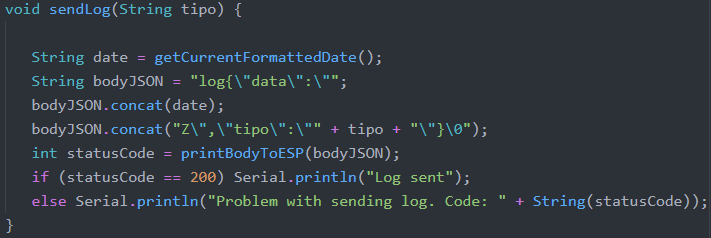
\includegraphics[width=0.99\linewidth]{./img/uno_log.png}
		\caption{Funzione per mandare un log all'ESP-01}
		\label{fig:uno_log}
	\end{subfigure}
	\caption{Snippet di codici caricati sull'Arduino UNO}
	\label{fig:uno_functions}
\end{figure}

In base alla richiesta vengono attivate 2 funzioni diverse:

\begin{itemize}
	\item una per mandare la verifica del tag al server (Figura \ref{fig:esp_check})
	\item una per mandare il log al server (Figura \ref{fig:esp_log})
\end{itemize}

\begin{figure}
	\centering
	\begin{subfigure}{0.5\textwidth}
		\centering
		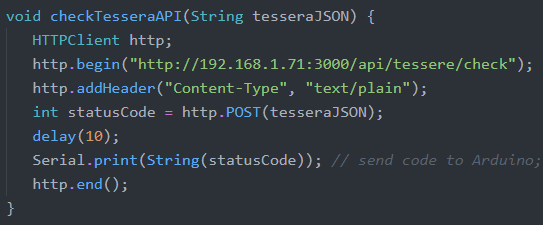
\includegraphics[width=0.95\linewidth]{./img/esp_check.png}
		\caption{Funzione per mandare la verifica del tag al server tramite una chiamata HTTP}
		\label{fig:esp_check}
	\end{subfigure}%
	\begin{subfigure}{0.5\textwidth}
		\centering
		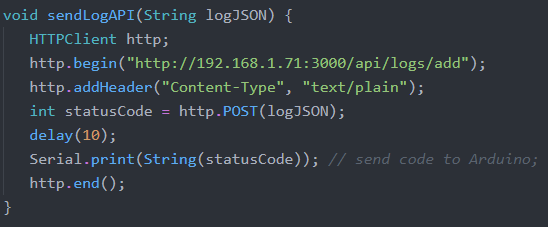
\includegraphics[width=0.95\linewidth]{./img/esp_log.png}
		\caption{Funzione per mandare il log al server tramite una chiamata HTTP}
		\label{fig:esp_log}
	\end{subfigure}
	\caption{Snippet di codici caricati sull'ESP-01}
	\label{fig:esp_functions}
\end{figure}

\subsection{Comunicazione tra l'Arduino UNO e l'ESP-01 }

L'Arduino UNO è programmato per comunicare con l'ESP-01 tramite SoftwareSerial (https://www.arduino.cc/en/Reference/SoftwareSerial), una libreria che replica, per via software, le funzionalità della comunicazione seriale hardware (sui pin 0 e 1) anche su altri pin digitali. Un esempio di inizializzazione si può trovare in Figura \ref{fig:arduino_esp_serial_setup}.


\begin{figure}
	\center{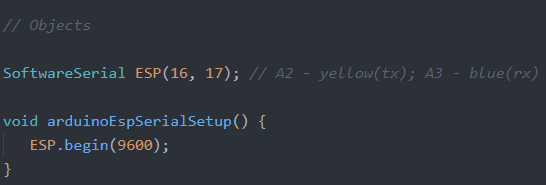
\includegraphics[width=0.6\linewidth]{./img/arduino_esp_serial_setup.png}}
	\caption{Snippet del codice per il setup della comunicazione seriale tra l'ESP-01 e l'Arduino UNO}
	\label{fig:arduino_esp_serial_setup}
\end{figure}

Come si è visto nelle Figure \ref{fig:esp_check} e \ref{fig:esp_log}, l'Arduino inoltra all'ESP-01 delle stringhe che sono quasi in formato JSON: prima dell'oggetto JSON c'è un'altra stringa usata per identificare la funzione voluta (e.g. "check{object}" e "log{object}"). L'ESP-01 poi filtra questi dettagli non piu' necessari (come in Figura \ref{fig:esp01_listen}) e chiama la funzione richiesta.

Esempio che descrive gli eventi per la verifica del tag:

\begin{enumerate}
	\item L'utente avvicina il tag al lettore RFID
	\item L'Arduino legge il seriale del tag e chiama "checkCardSerial(serial)"
	\item Questa funzione manda un'oggetto in formato quasi-JSON all'ESP-01
	\item L'ESP-01 riceve questa stringa e filtra l'informazione non piu' necessaria
	\item L'ESP-01 chiama la funzione richiesta (in questo caso "checkTesseraAPI(serialeJSON)")
	\item La funzione eseguita manda l'oggetto JSON al server e aspetta una risposta con lo status code.
	\item L'ESP-01 inoltra lo status code all'Arduino
	\item In base allo status code l'Arduino prende una decisione: se statusCode = 200 allora il tag è accettato e l'Arduino apre la porta, altrimenti viene rifiutato.
\end{enumerate}

Come si può vedere dalla sequenza degli eventi, l'ESP-01 non è altro che un middleman tra l'Arduino e il server.
%
\section{Protocolli di trasmissione dati}
%


%
\subsection{Logica IoT}
%
WiFi

%
\subsection{I$^2$C}\label{sec:i2c}
%

%
\subsection{SPI}\label{sec:spi}
% 
%			CAPITOLO 3: Software
\chapter{Software}
\label{cap3}
%
%
%
\section{Strumenti dello sviluppatore}
Arduino IDE
\\
Node.js
\\
Postman
\\
MongoDB 
\\
Per i linguaggi di programmazione metto solo un riferimento alla bibliografia
%
%
\section{Sviluppo del sistema embedded}
Snippet e spiegazioni di codice
\\

%
%
\section{Sviluppo dell'interfaccia web}
%
\subsection{Back-End}
\subsection*{Scelte progettuali}
MVC
\subsection*{Database}
%
\subsection*{API}
Documentazione delle API del back-end
%
\subsection{Front-End}
\subsection*{Scelte progettuali}
Le basi: Javascript, HTML5 \& CSS
\\
w3.css
\\
jQuery
\\
EJS
\\
%
% 
%			CAPITOLO 4: Analisi del progetto
\chapter{Analisi del progetto}
\label{cap4}
Prestazioni
\\
Problema sicurezza
\\
Possibili miglioramenti
\\
%
% 
%			CAPITOLO 5: Conclusioni
\chapter{Conclusioni}


\label{cap5}
%
%

\appendix
\chapter{Una prima Appendice (?)}
...

%
%			BIBLIOGRAFIA
%
\begin{thebibliography}{00}
	

\bibitem{controllo_accessi}
J. Allen, Opening new doors with IP access control, 16 Marzo, 2018. \url{https://www.axis.com/blog/secure-insights/opening-new-doors-with-ip-access-control/}
%

\bibitem{crescita_controllo_accessi}
R. Alalouff, Access control leads growth in physical security market but video surveillance still dominates, 25 Gennaio, 2018.
\url{https://www.ifsecglobal.com/access-control/access-control-leads-growth-physical-security-market-video-surveillance-still-dominates/}
%
\bibitem{smart_objects}
A. Tumino, Internet of Things: gli oggetti intelligenti prima di ogni "cosa", 24 Gennaio, 2018.
\url{https://blog.osservatori.net/it_it/internet-of-things-oggetti-intelligenti-prima-di-ogni-cosa}
%
\bibitem{IoT}
M. Rouse, Internet of Things (IoT), ultimo aggiornamento Marzo 2019.
\url{https://internetofthingsagenda.techtarget.com/definition/Internet-of-Things-IoT}
% 
\bibitem{arduino_storia}
Arduino, Un po' di storia.
\url{https://playground.arduino.cc/Italiano/StoriaDiArduino/}
%

\bibitem{sistemi_embedded_atrent}
A. Carraturo, A. Trentini, Sistemi Embedded: Teoria e Pratica, prima edizione: Settembre 2017.
\url{http://www.ledizioni.it/prodotto/a-carraturo-a-trentini-sistemi-embedded-teoria-pratica/}
%

\end{thebibliography}
%
\end{document}


 
